\documentclass[11pt]{article}

\usepackage{float} % [H] option for tables
\usepackage{booktabs} % table ruling
\usepackage{amssymb}
\usepackage{fullpage} % Use the full page
\usepackage{color}
\usepackage{tikz}
\usepackage[framed]{matlab-prettifier} % Matlab
\setlength\parindent{0pt} % No indentation


% Headers
\usepackage{fancyhdr}
\setlength{\headheight}{15.2pt}
\pagestyle{fancy}
\setlength\headsep{30pt}
\lhead{Youssef Beltagy and Samuel Hunter}   					%  Your name on the left header.
\chead{\textsc{Lab 4}}			%  Title in the center.
\rhead{\today}							%  Date on the right header.

% Matlab blocks
\lstset{
  style              = Matlab-editor,
  basicstyle         = \mlttfamily,
  mlshowsectionrules = true,
  escapeinside={//}{//},
}

% Cover Page Settings
\title{
    \textsc{Lab 4 Report: Frequency-Domain Signal Filtering}
}

\author{
    \Large{Youssef Beltagy and Samuel Hunter} \\
    \large \textsc{AUT21 BEE 235}
}

\date{\today}

%--------------------------------------------
%%%%%%%%%%%%%%%%%%%%%%%%%%%%%%%%%%%%%%%%%%%%%%%%%%%%
% END OF THE PREAMBLE AND BEGINNING OF THE ACTUAL DOCUMENT
%%%%%%%%%%%%%%%%%%%%%%%%%%%%%%%%%%%%%%%%%%%%%%%%%%%%
%--------------------------------------------

\begin{document}


\maketitle % Make the cover page
\pagebreak


\section{Abstract}

In this lab, we used the fourier transform of a signal
to filter it. We observed how low pass, high pass, and band pass filters affect the signal.
We listened to the difference in sound and observed the change in the time and frequency domain plots.

\section{Exercise 1 --- Low Pass Filter}

We used Fourier Transform to analyze a sound signal.
We multiplied the signal spectrum with $\frac{500}{500 + j \cdot \omega}$
to run it through a low pass filter (LPF). We then used the inverse fourier transform to 
synthesize the new signal.\\

The filtered signal sounds quieter and duller than the original signal.
It sounds muffled.\\

Visually, the filtered time-domain signal is clearly missing some high frequency
components between times 2 and 3. The filtered frequency-domain signal 
lost all its higher frequency values.

\subsection{Output}

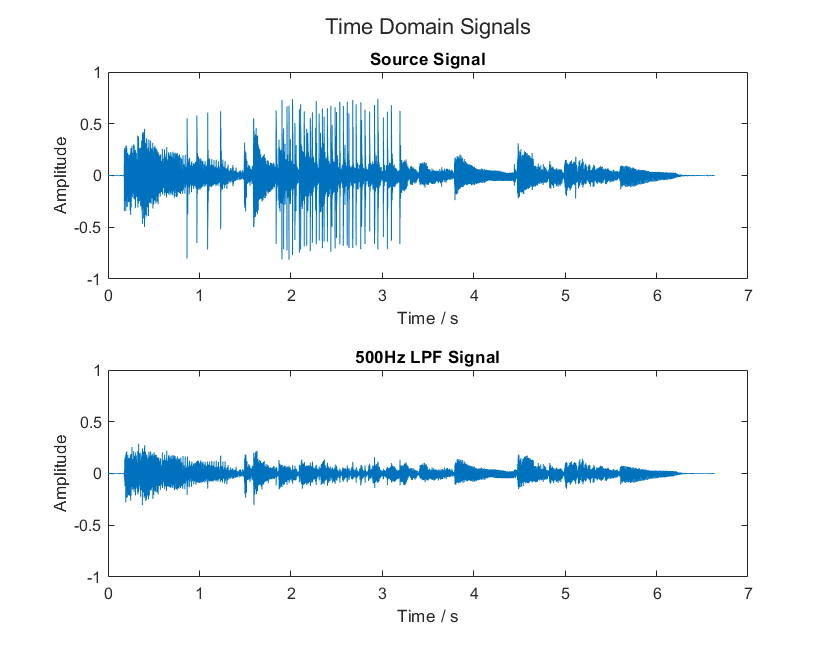
\includegraphics[height=0.5\textheight]{lpf_time.png}

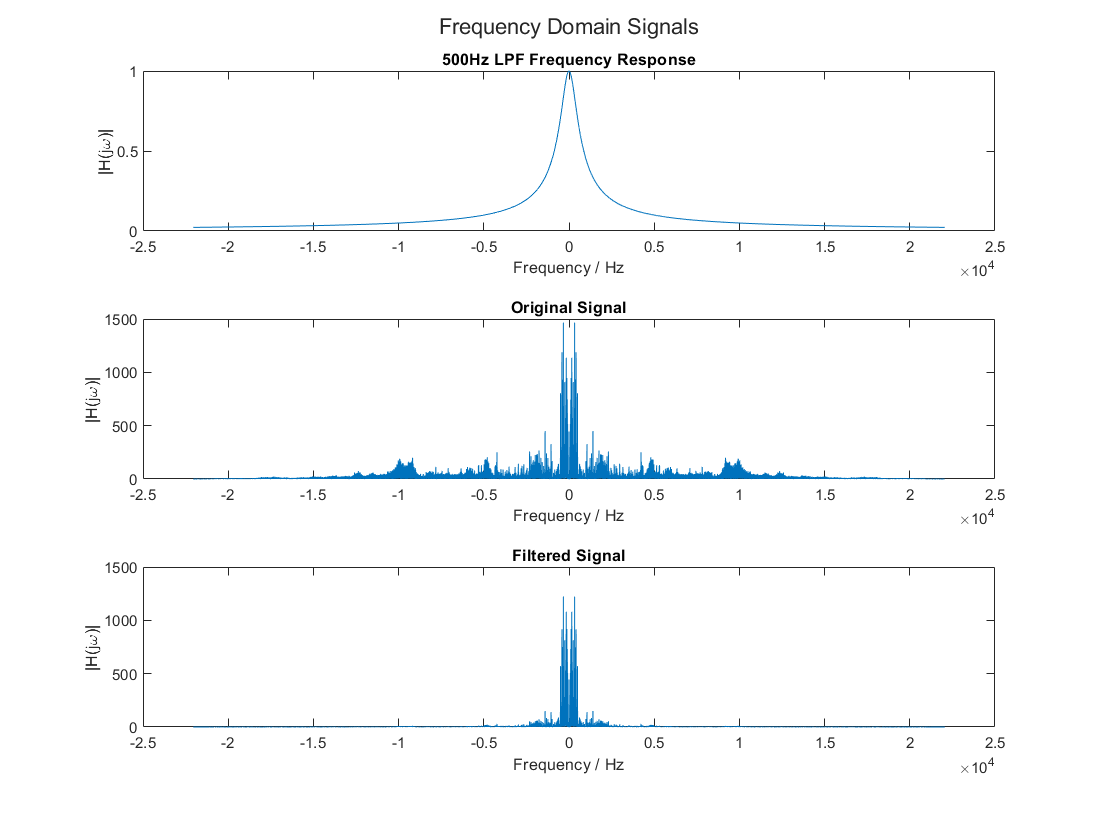
\includegraphics[height=0.5\textheight]{lpf_frequency.png}

\subsection{Code}
We modularized loading the data, filtering, plotting, and playing the sound.
First, we load the data.

\lstinputlisting{LoadData.m}

Then, we run the filtering logic.

\lstinputlisting{SignalLowPass.m}

Then, we plot the results.

\lstinputlisting{PlotSignals.m}

Lastly, we play the sounds.

\lstinputlisting{PlaySignals.m}

\section{Exercise 2 --- High Pass Filter}

We repeated exercise 1 but with a high pass filter (HPF).
The HPF makes the signal sound sharp but far away.\\

Visually, the time-domain filtered signal lost 
what seems like a DC component part of the signal. 
For example, from 0 to 1 seconds, the filtered signal has lower
average amplitudes even though it seems to have the same maximum amplitude.
This is likely what they call bass.\\

The frequency domain filtered signal clearly lost its
lower frequency values. The two towers next to the 0 are gone. 
But the higher frequency values remain unchanged.

\subsection{Output}

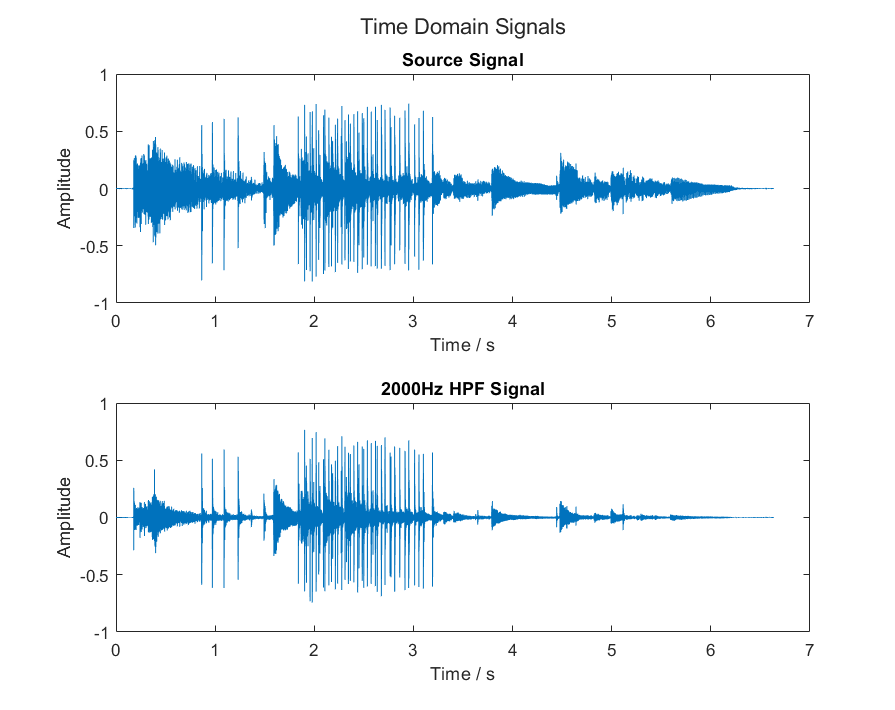
\includegraphics[height=0.5\textheight]{hpf_time.png}

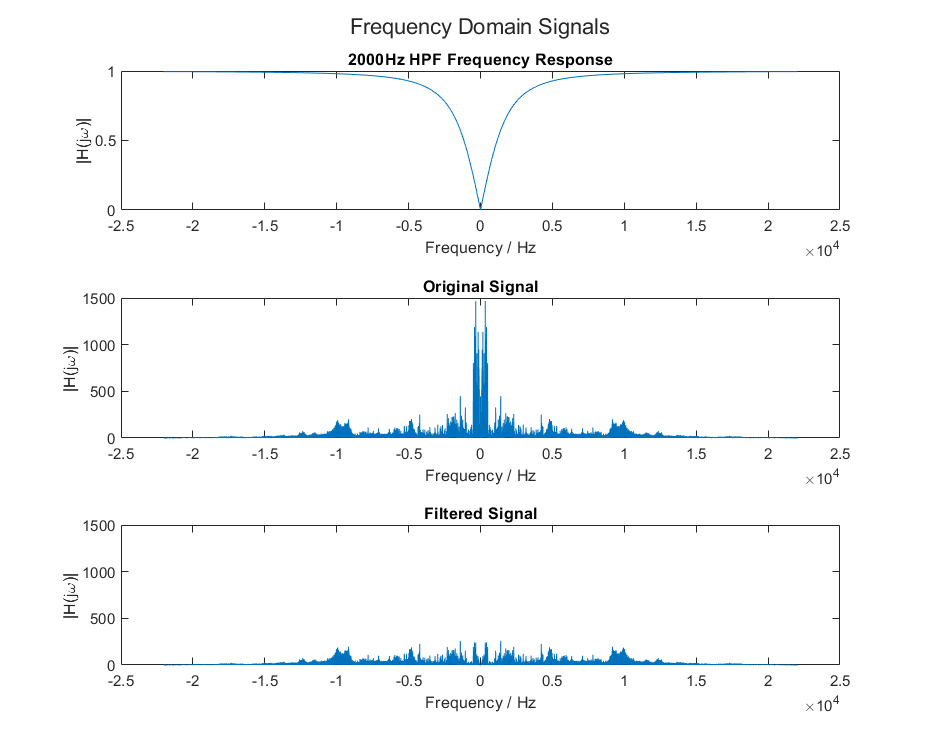
\includegraphics[height=0.5\textheight]{hpf_frequency.png}

\subsection{Code}

\lstinputlisting{SignalHighPass.m}

\section{Exercise 3 --- Band Pass Filter}

We combined exercises 1 and 2 to make a band pass filter (BPF).
This signal didn't sound significantly different from the original 
signal.\\

Visually, the filtered time-domain signal retained its form. 
But it is weaker. It lost some of its bass components just
like the HPF but its high frequency components from seconds 1 to 2
became weaker as well. It looks like a combination of the LPF and HPF
(it is).\\

The frequency-domain signal lost its highest frequency components.
The lower frequency components (the two towers) became much weaker. 

\subsection{Output}

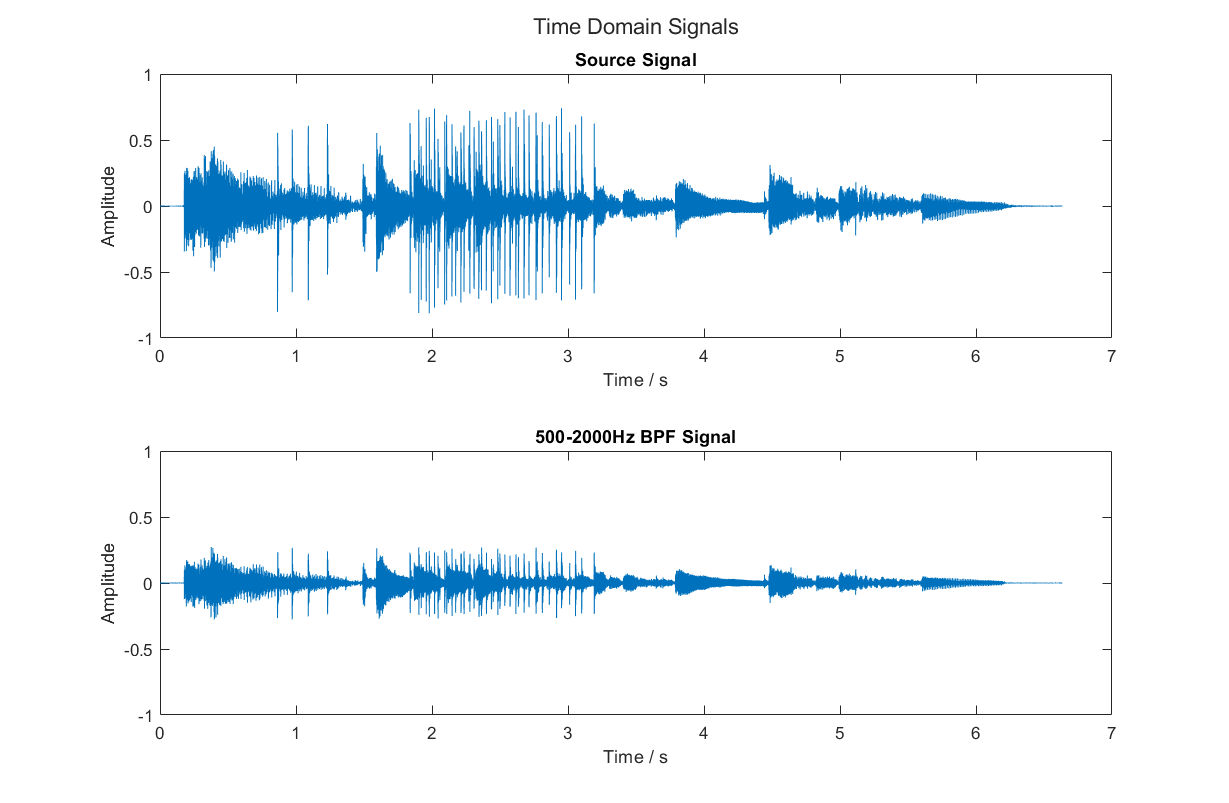
\includegraphics[width=\textwidth]{bpf_time.png}

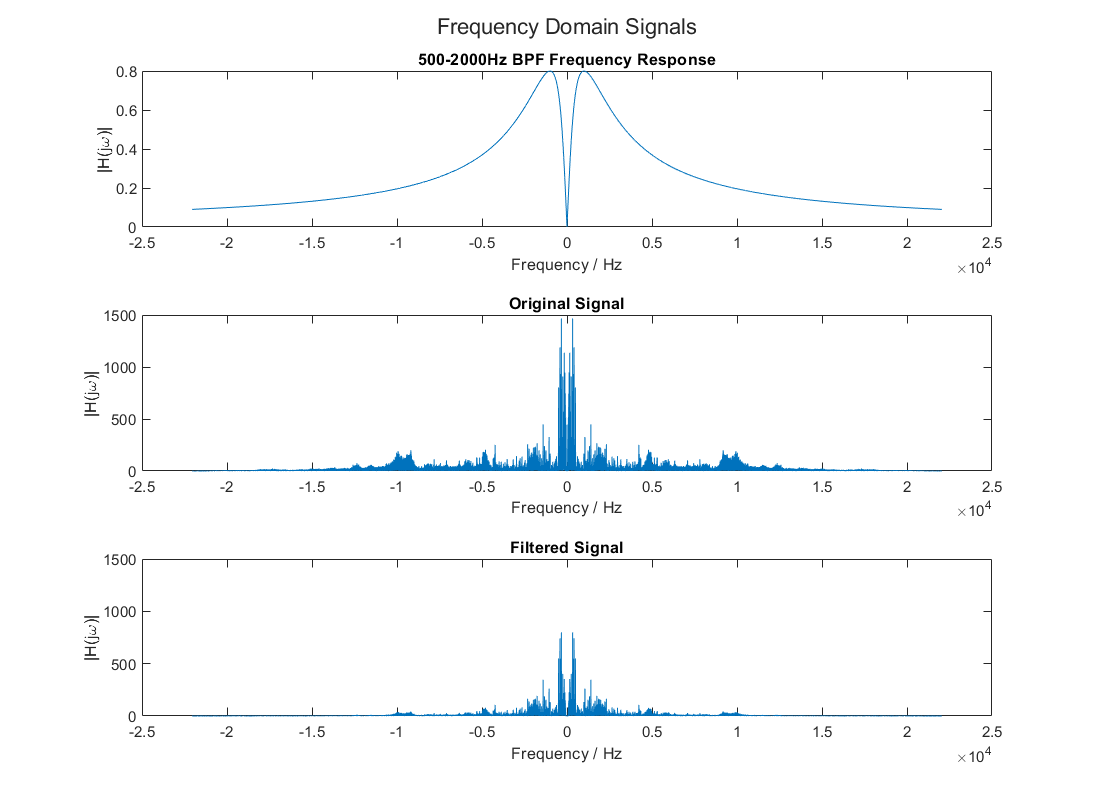
\includegraphics[width=\textwidth]{bpf_frequency.png}

\subsection{Code}

\lstinputlisting{SignalBandPass.m}

\section{Conclusion}

Filters can be implemented by analyzing the fourier transform of 
a signal and multiplying it by the frequency response of a filter.
This process is straightforward and effective.\\

The effects of filters is easy to notice in both the time and frequency domains.

\end{document}
